
\section{Xây dựng hệ thống xử lý ảnh}

\subsection{Pipeline xử lý ảnh}
Hệ thống kiểm tra ngoại quan tự động (Automated Visual Inspection – AVI) vận hành thông qua một chuỗi các bước xử lý ảnh được tổ chức theo dạng pipeline nhằm đảm bảo quá trình kiểm tra diễn ra chính xác, ổn định và nhất quán. Pipeline xử lý ảnh của hệ thống có thể được mô tả qua các giai đoạn chính như sau:

\subsubsection{Thu nhận hình ảnh}
Ở giai đoạn đầu tiên, camera độ phân giải cao hoặc thiết bị ghi hình chuyên dụng được sử dụng để thu nhận ảnh hoặc video của sản phẩm. Chất lượng ảnh đầu vào phụ thuộc vào loại camera, ống kính, khoảng cách chụp và cấu hình hệ thống chiếu sáng. Đây là nguồn dữ liệu cơ bản phục vụ toàn bộ quá trình xử lý phía sau.

\subsubsection{Xử lý và tiền xử lý hình ảnh}
Sau khi thu nhận, hình ảnh được đưa vào các thuật toán xử lý nhằm tăng cường chất lượng, làm nổi bật đặc trưng quan trọng và giảm nhiễu. Các bước thường bao gồm:
\begin{itemize}
    \item Cân bằng sáng, tăng tương phản hoặc hiệu chỉnh màu.
    \item Lọc nhiễu và cải thiện độ nét.
    \item Chuẩn hóa kích thước, góc xoay hoặc cắt vùng quan tâm (ROI).
\end{itemize}
Giai đoạn này đảm bảo rằng hình ảnh đầu vào luôn đạt chất lượng ổn định để phục vụ nhận diện lỗi.

\subsubsection{Phân tích ảnh và nhận diện lỗi}
Ở bước này, hệ thống áp dụng các thuật toán xử lý ảnh nâng cao và mô hình học máy để:
\begin{itemize}
    \item Trích xuất đặc trưng của sản phẩm.
    \item Phát hiện các bất thường hoặc khuyết tật như vết nứt, thiếu linh kiện, sai lệch vị trí, biến dạng hình học.
    \item So sánh với hình mẫu hoặc tiêu chuẩn kỹ thuật đã thiết lập.
\end{itemize}
Thuật toán AI và machine learning giúp hệ thống thích nghi với biến động trong môi trường sản xuất, từ đó cải thiện độ chính xác theo thời gian.

\subsubsection{Ra quyết định}
Dựa trên các tiêu chí chất lượng đã định nghĩa trước, hệ thống phân loại sản phẩm thành hai nhóm: đạt yêu cầu (OK) hoặc không đạt (NG). Việc ra quyết định được tự động hóa và đảm bảo tính khách quan, loại bỏ hoàn toàn yếu tố chủ quan của con người.

\subsubsection{Phản hồi và lưu trữ dữ liệu}
Kết quả kiểm tra được ghi nhận và phản hồi trực tiếp đến hệ thống sản xuất để thực hiện các hành động kịp thời như loại bỏ sản phẩm lỗi hoặc điều chỉnh quy trình. Đồng thời, dữ liệu hình ảnh, log lỗi và thống kê được lưu trữ trên cơ sở dữ liệu cục bộ hoặc đám mây để phục vụ phân tích chất lượng, tối ưu hoá dây chuyền và truy vết trong sản xuất.

Pipeline trên giúp hệ thống AVI hoạt động mạch lạc, hiệu quả và có khả năng mở rộng theo yêu cầu thực tế của từng dây chuyền sản xuất.

\subsection{Train mô hình YOLO detect linh kiện SMD}

\subsubsection{Thu thập dữ liệu}
Ảnh được thu thập trực tiếp từ camera trong dây chuyền bằng cách chụp nhiều mẫu PCB ở nhiều điều kiện khác nhau: thay đổi độ sáng, vị trí, góc đặt bảng, và trạng thái linh kiện (đầy đủ hoặc lỗi). Mục tiêu là tạo bộ dữ liệu đa dạng, phản ánh đúng môi trường sản xuất thực tế để mô hình học sâu có khả năng tổng quát tốt.

\begin{figure}[H]
    \centering
    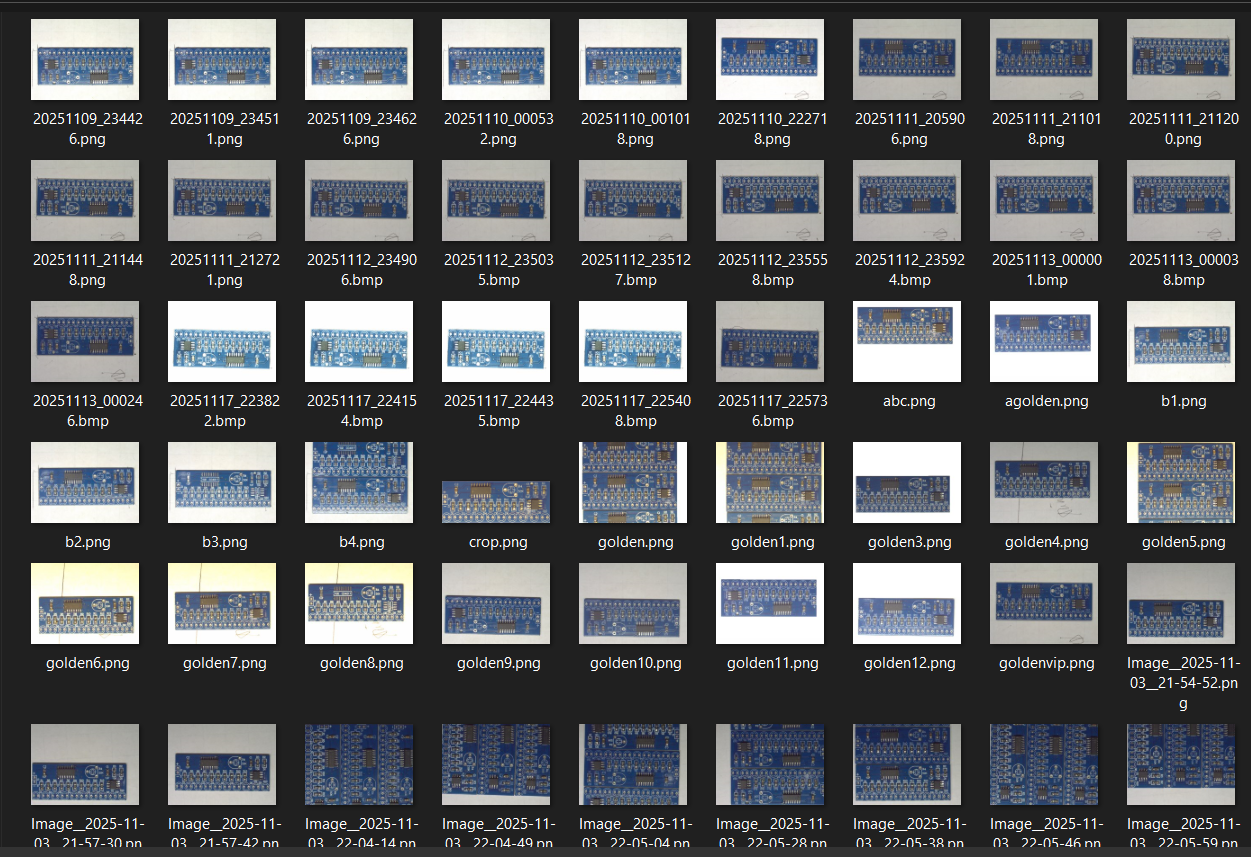
\includegraphics[width=0.75\linewidth]{figures/Chapter3/image11.png}
    \caption{Thu thập ảnh}
    \label{c3:acquistion}
\end{figure}

\subsubsection{Gán nhãn dữ liệu (Labeling)}
Sau khi thu thập, toàn bộ ảnh được đưa vào nền tảng Roboflow để thực hiện gán nhãn. Mỗi linh kiện SMD hoặc vùng lỗi trên PCB được bao quanh bằng bounding box và gán class tương ứng, chẳng hạn như \texttt{OK}, \texttt{Missing}, \texttt{Shifted}, \texttt{Wrong\_Orientation}, \ldots{} Việc gán nhãn được thực hiện thủ công nhằm đảm bảo độ chính xác, vì chất lượng nhãn có ảnh hưởng trực tiếp đến khả năng học của mô hình YOLO.

Roboflow hỗ trợ việc chuẩn hoá kích thước ảnh, tăng cường dữ liệu (augmentation) như xoay, thay đổi độ sáng, cắt, lật ảnh, giúp tăng độ đa dạng cho tập huấn luyện. Sau khi hoàn tất, bộ dữ liệu được export theo định dạng YOLO và sẵn sàng cho quá trình huấn luyện.
\begin{figure}[H]
    \centering
    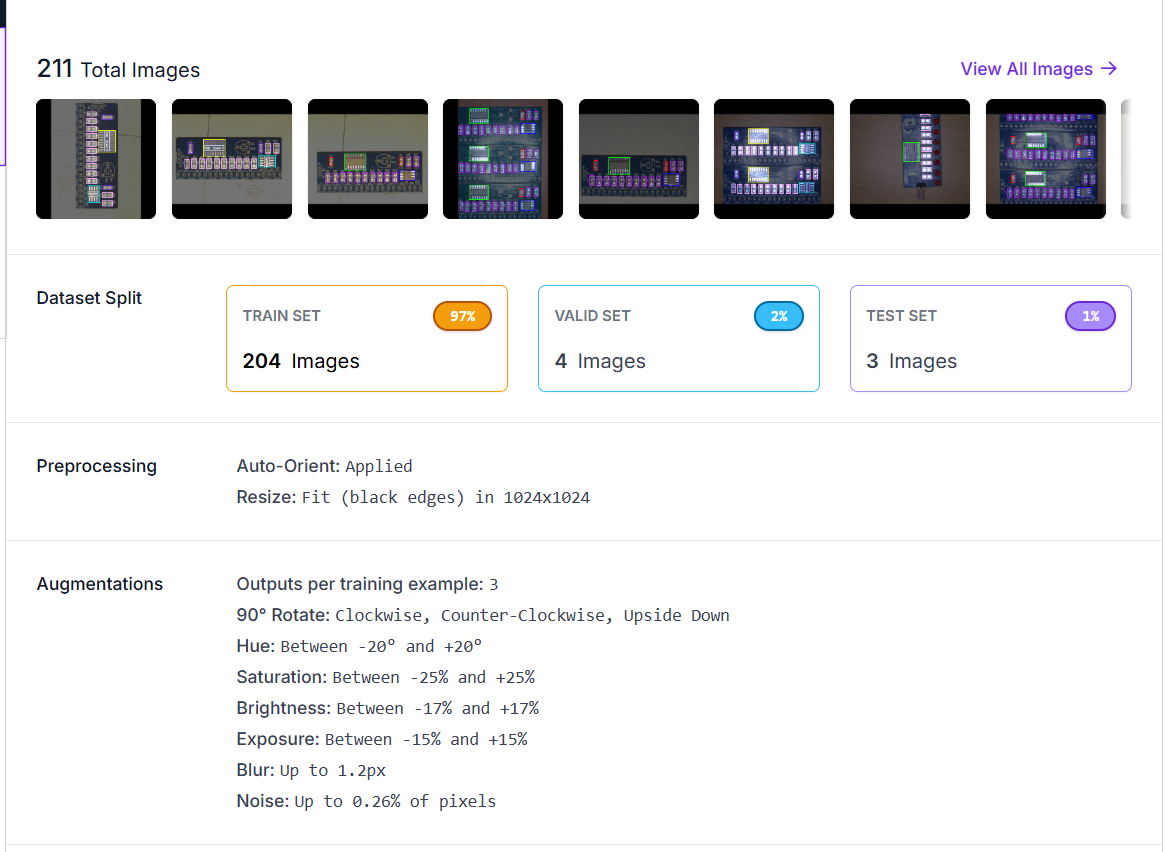
\includegraphics[width=0.75\linewidth]{figures/Chapter3/image12.png}
    \caption{Label ảnh bằng Roboflow}
    \label{c3:labeling}
\end{figure}

\subsubsection{Huấn luyện mô hình (Train model)}
Bộ dữ liệu sau khi export được đưa lên môi trường Google Colab để huấn luyện mô hình YOLO. Colab cung cấp GPU miễn phí, phù hợp cho huấn luyện nhanh các mô hình kích thước vừa.

Quy trình huấn luyện gồm các bước:
\begin{itemize}
    \item Upload bộ dữ liệu từ Roboflow vào Colab bằng API.
    \item Cấu hình file huấn luyện: đường dẫn dữ liệu, số lớp (classes), độ phân giải ảnh, batch size, và số epochs.
    \item Tiến hành huấn luyện và theo dõi các chỉ số: loss, precision, recall, mAP.
    \item Lưu lại \texttt{best.pt} sau khi huấn luyện, sử dụng cho giai đoạn suy luận (inference) trong hệ thống AVI.
\end{itemize}

Mô hình sau khi huấn luyện được tải xuống và đưa vào pipeline xử lý ảnh để thực hiện phát hiện linh kiện SMD trong thời gian gần thực.

